\documentclass[12pt,a4paper]{article}
\usepackage[utf8]{inputenc}
\usepackage[french]{babel}
\usepackage[T1]{fontenc}
\usepackage{amsmath}
\usepackage{amsfonts}
\usepackage{amssymb}
\usepackage{makeidx}
\usepackage{graphicx}
\usepackage{lmodern}
\usepackage{index}
%\usepackage{hyperref}
\newcommand{\HRule}{\rule{\linewidth}{0.5mm}}
%\usepackage{kpfonts}
\usepackage{fourier}
\usepackage[left=2cm,right=2cm,top=2cm,bottom=2cm]{geometry}
\author{Sarah Kaddah}
\title{Rapport de stage}

%%%%%%%%%%Interligne
\renewcommand{\baselinestretch}{1.5}
\begin{document}
%%%%%%%%%%%%%%%%%%%%%%%%%%%%%%%%%%%%%%%%%%%%%%%%%%%%%%%%%%%%%%%%%
%%%%%%%%%%%%%%%%%%%%%%1ere page%%%%%%%%%%%%%%%%%%%%%%%%%%%%%%%%%%
%%%%%%%%%%%%%%%%%%%%%%%%%%%%%%%%%%%%%%%%%%%%%%%%%%%%%%%%%%%%%%%%%
%%%%%%%%%%%%%%%%%%%%%%%%%%%%%%%%%%%%%%%%%%%%%%%%%%%%%%%%%%%%%%%%%
\begin{titlepage}
  \begin{sffamily}
  \begin{center}
	\large{Master 2 Biologie-Informatique/ Bioinformatique \hfill 2017-2018}
	\flushleft{\large{Université Paris Diderot - Paris 7}}
	
%	\begin{center}
%		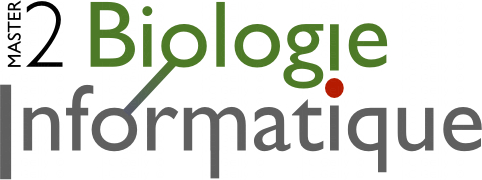
\includegraphics[scale=0.3]{img/m2.png} \hfill
%		
\includegraphics[scale=0.1]{img/p7.png}
%	\end{center}

\begin{tabular}{c}
\\ \\ \\
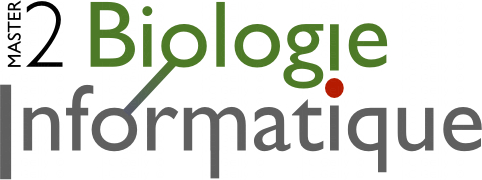
\includegraphics[scale=0.3]{img/m2.png}
\end{tabular}
\hfill
\begin{tabular}{c}
\\

\includegraphics[scale=0.1]{img/p7.png}
\end{tabular}

%%%%%%%%% Title    
    \HRule \\[0.2cm]
    { \huge \bfseries \center{Etude de la fonction et des mécanismes d'évolution des séquences répétées centromériques chez les Primates}\\[0.4cm] }
    \HRule \\[2cm]
%%%%%%%%Centre de la page    
\begin{center}\LARGE{\textbf{Sarah Kaddah}}\end{center}
\begin{center}\Large{Tuteur: Lo\"{i}c Ponger}\end{center}~\\[0.5cm]
%%%%%%%%% Bottom of the page
\center{\large{Structure et Instabilité des Génomes}}
\center{\large{ MNHN - CNRS UMR 7196 / INSERM U1154 - Sorbonne Universités}}\\[1cm]

%	\begin{center}
%		
\includegraphics[scale=0.2]{img/mnhn.jpg} \hfill
%		
\includegraphics[scale=0.08]{img/cnrs.png} \hfill
%		
\includegraphics[scale=0.08]{img/inserm.jpg}
%	\end{center} 

\begin{tabular}{cc}
 \hspace*{3cm} &  

\includegraphics[scale=0.2]{img/mnhn.jpg}
\end{tabular}
\hfill
\begin{tabular}{c}

\includegraphics[scale=0.08]{img/inserm.jpg}
\end{tabular}
\hfill
\begin{tabular}{cc}

\includegraphics[scale=0.08]{img/cnrs.png} &
\hspace*{3cm}
\end{tabular}

%%%%%%%%% END
  \end{center}
  \end{sffamily}
\end{titlepage}
%%%%%%%%%%%%%%%%%%%%%%%%%%%%%%%%%%%%%%%%%%%%%%%%%%%%%%%%%%%%%%%%%%
%%%%%%%%%%%%%%%%%%%%%Remerciements%%%%%%%%%%%%%%%%%%%%%%%%%%%%%%%%
%%%%%%%%%%%%%%%%%%%%%%%%%%%%%%%%%%%%%%%%%%%%%%%%%%%%%%%%%%%%%%%%%%
\thispagestyle{empty}
\section*{\begin{center}Remerciements\end{center}}~\\[0.2cm]
\addcontentsline{toc}{section}{Remerciements}
Merci à Namrod pour toute la partie sur la bibliographie. Retrouvez ses questions FAQ qui ont permis la rédaction de cette partie.\\
\noindent Merci à f-leb, LittleWhite et Metalman pour leurs conseils et la relecture.
\noindent Merci à ced et jacques\_jean pour la correction orthographique et typographique.


%%%%%%%%%%%%%%%%%%%%%%%%%%%%%%%%%%%%%%%%%%%%%%%%%%%%%%%%%%%%%%%%%%
%%%%%%%%%%%%%%%%%%%Table des matières%%%%%%%%%%%%%%%%%%%%%%%%%%%%
%%%%%%%%%%%%%%%%%%%%%%%%%%%%%%%%%%%%%%%%%%%%%%%%%%%%%%%%%%%%%%%%%

\newpage
\tableofcontents
\setcounter{page}{0}
\newpage 
%%%%%%%%%%%%%%%%%%%%%%%%%%%%%%%%%%%%%%%%%%%%%%%%%%%%%%%%%%%%%%%%
%%%%%%%%%%%%%%%%%%%%Introduction%%%%%%%%%%%%%%%%%%%%%%%%%%%%%%%%
%%%%%%%%%%%%%%%%%%%%%%%%%%%%%%%%%%%%%%%%%%%%%%%%%%%%%%%%%%%%%%%% 

\section{Introduction}
\subsection{Les séquences centromériques}
-> biblio CENP-A\\
-> biblio kinetochore\\
-> info supp sur l'ADN satellite\\

Le centromère est une structure chromatinienne caractérisé par la présence de CENP-A. Cette protéine, très conservée au cours de l'évolution, est un variant de l'histone H3. Son rôle est de fixer la position du kinétochore par un mécanisme encore peu connu. En effet, le centromère est le site d'assemblage du kinétochore, un ensemble d'ADN et de protéines. Il permet l'attachement du fuseau mitotique pour la ségrégation des chromosomes durant la division cellulaire chez les eucaryotes. Le centromère et les protéines impliquées sont relativement bien conservés. Au contraire, l'ADN sous-jacent est très diversifié et l'organisation varie d'un taxon à l'autre. Cependant, une caractéristique commune est retrouvée chez toute les espèces: de l'ADN centromérique répété en tandem nommé ADN satellite. Ces répétitions sont issues d'événements d'amplification, tels les crossovers inégaux, la conversion de gènes, les cercles roulants ou la transposition de séquences.[Malik and Henikoff, 2002; Plohl et al. 2012]
Ces séquences représentent 5\% du génome. Les répétitions s'étendent de 7pb à 3,2kb avec des séquences de 145-180kb le plus souvent.  

\subsection{L'ADN $\alpha$-satellites}
-> première mise en évidence des AS\\
->théorie gradient de l'âge\\
-> travaux sur le gorille à dev\\

L'ADN satellite chez les Primates est connu sous le nom d'$\alpha$-satellite. Ces séquences centromériques répétées en tandem sont riches en AT. 
-> article sur la première découverte

Des études chez l'Homme propose un modèle évolutif. La répartition des $\alpha$-satellites suivrait une répartition spécifique selon l'âge des familles. Les familles les plus jeunes s'insèrent au cœur du centromère, repoussant les familles les plus anciennes jusqu'aux regions voisines, appelé péri-centromère.\\
->Article Shepelev\\
->Est-ce que je peux utiliser du conditionnel? OU est-ce que cette théorie est confirmée?

Un monomère a une longueur de 171pb et il peut être répété des milliers de fois. Les monomères peuvent être répartis en famille selon leur similarité, les séquences ayant un taux d'identité supérieur à 70\%. Ces séquences ont soit une organisation monomérique soit une organisation en répétition d'ordre supérieur (Fig. 1). Dans le premier cas, les séquences d'une même famille sont répétés en tandem. Dans le deuxème cas, une suite de monomères appartenant à différentes familles forme une unité, qui elle est répétée en tandem. 



Ces séquences peuvent avoir un site de liaison à la protéine centromérique CENP-B un motif spécifique de 17pb. Cette protéine, qui reconnaît et se fixe sur l'ADN, serait présente chez de nombreuses familles de Primates. La protéine pJ$\alpha$, une protéine peu caractérisée, reconnaît un motif qui remplace celui de CENP-B.

Les $\alpha$-satellites ont essentiellement été étudiées chez l'homme. Modèle évolutif avec les centromères en expansion. Une hypothèse concernant l'âge des séquences découle de ces recherches: les séquences les plus récentes apparaissent au coeur du centromères, déplançant les plus anciennes au péricentromère. D'autres études chez le gorille ont été faites. Le rôle des $\alpha$-satellites est encore mal connu. 

\begin{figure}
	\center
		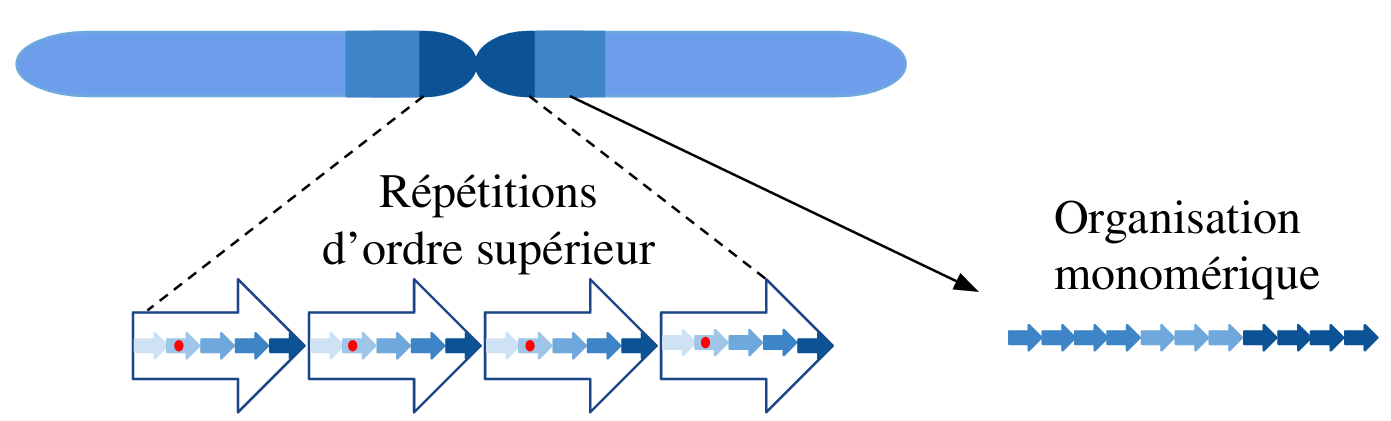
\includegraphics[height=3.5cm, width=12cm]{img/AS_organization.png}
		\caption{\textbf{Organisation spatiale des $\alpha$-satellites:} Le coeur du centromère (bleu foncé) est organisé en répétition d'ordre supérieur. Le péricentromère(bleu clair) a une organisation monomérique. Un monomère d'une même famille est représenté par une petite flèche de même couleur. Les points rouges représentent les sites de fixation à CENP-B ou pJ$\alpha$.}
\end{figure}


\subsection{Le sujet de stage}
enchaîne sur l'étude chez les cerco, une autre étude de séquençage haut débit\\

-travaux précédents limités (expliquer pk). Les méthodes basées aur l'alignement et la phylogénie sont très limitées, le jeu de données étant trop grand. Les méthodes n'étaient pas objectives (quelles méthodes??). De plus, chez d'autres espèces de Primates, les informations sont trop dispersées et aucune comparaison interespèce n'a été faite. \\


L'équipe d'accueil de mon stage "ADN répété, Chromatine, Evolution" ou ARChE, a récemment développé une approche de séquençage haut débit, ciblée sur les séquences $\alpha$-satellites chez deux espèces de Cercopithèques. Une autre étude avec un grand nombre de séquences concerne le Gorille [Catacchio] avec l'utilisation de fragments relativement longs. 

L'objectif de ce stage est de comprendre la fonction des $\alpha$-satellites et leur mécanisme d'évolution. Je vais choisir plusieurs espèces de Primates. Je vais utiliser une méthode de classification automatisée améliorée du laboratoire [Florence Jornod] pour classer les séquences en familles.  Ce programme permet de traiter des centaines de milliers de séquences sans quelque soit le nombre de séquences ou la taille des familles. Je vais dans un premier temps appliquer cette technologies au données issues de ce séquençage. Ensuite, je vais étudier d'autres espèces. Puisque toutes les espèces sont étudiées par la  même méthode, une comparaison inter espèce est envisageable. 

%%%%%%%%%%%%%%%%%%%%%%%%%%%%%%%%%%%%%%%%%%%%%%%%%%%%%%%%%%%%%%%%%
%%%%%%%%%%%%%%%%%%%%%%M & M%%%%%%%%%%%%%%%%%%%%%%%%%%%%%%%%%%%%%%
%%%%%%%%%%%%%%%%%%%%%%%%%%%%%%%%%%%%%%%%%%%%%%%%%%%%%%%%%%%%%%%%% 
\section{Matériel et méthode}
\subsection{Choix des espèces}
Les critères de sélection dépendent de la disponibilité des séquences de qualité. Deux espèces du laboratoire sont choisies, les \textit{Cercopithèques solatus} et \textit{pogonias}, et deux espèces proches, le \textit{Macaca fascicularis} et le \textit{Chlorocebus sabaeus}.  
	\begin{figure}
		\center
		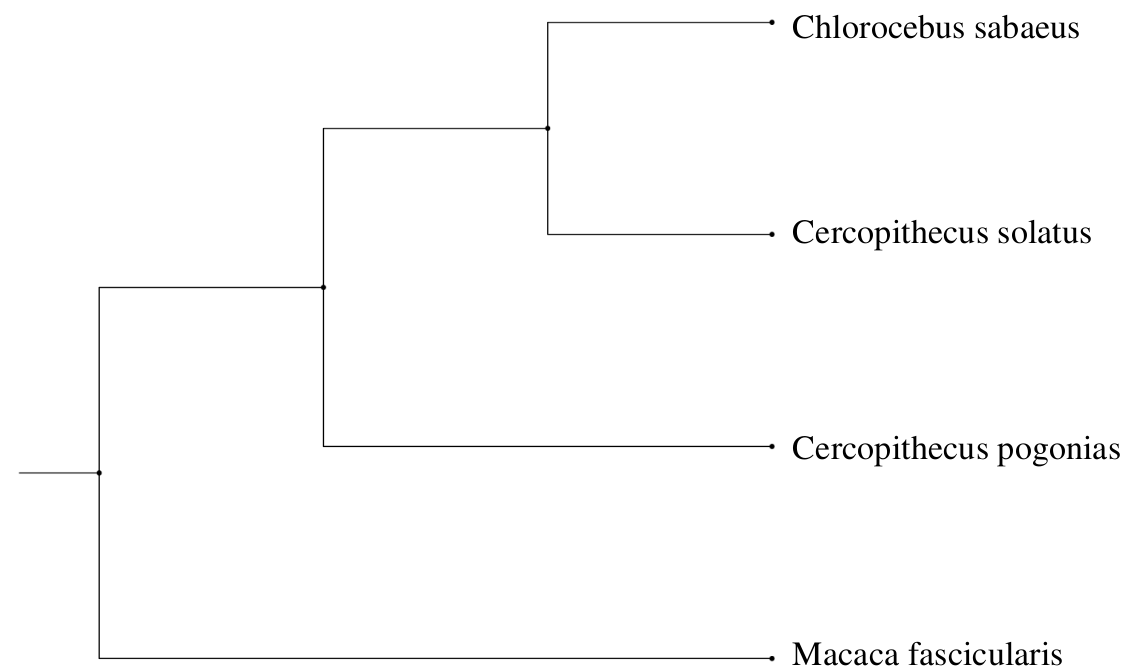
\includegraphics[height=4.5cm, width=7cm]{img/arbre_especes.png}
		\caption{\textbf{Arbre phylogénétique des espèces choisies.}}
	\end{figure}

\subsection{Méthode de classification}
	\subsubsection{Principe}
Cette méthode \cite{rapport_florence} répartit des séquences $\alpha$-satellites en familles selon la similarité. La classification est hiérarchique dichotomique. Au départ, une table de 5-mers est calculée pour chaque monomère.  Ensuite, toutes les séquences sont ajoutées dans la file. Ensutie une boucle itérative est exécutée pour séparer les séquences en groupes tant que les nouveaux groupes formés sont divisibles.
	\subsubsection{Répartition itérative}
Une Analyse en Composante Principale (ACP) est effectuée sur la table de fréquence des 5-mers afin de réduire les dimensions du jeu de données et d’obtenir des variables indépendantes. Des distances euclidiennes sont calculées entre toutes les paires de séquence dans l’espace défini par les M premières composantes de l’ACP. A partir du calcul de distance, les séquences sont séparées en deux classes en utilisant la classification hiérarchique basée sur la méthode de Ward. La classification hiérarchique permet de former des classer de façon à maximiser l’inertie interclasse. Cette étape fait un usage important de la mémoire. Par conséquent, pour traiter des jeux de données importants, l’Analyse Discriminante Linéaire , une méthode d’apprentissage, est utilisée sur un sous jeu de données formé par des séquences tirées aléatoirement. Le modèle construit est alors appliqué sur toutes les séquences.
	\subsubsection{Validation d'un sous-groupe}
L'étape suivante est une double validation des sous-groupes. D'une part la taille du sous-groupe est vérifiée. La taille minimale d'une famille est fixée à 100. Si un groupe atteint 100 séquences, il n'est pas redivisé. D'autre part les deux groupes doivent être distincts. Pour cela le \textit{matepair}, la proportion de monomères ayant son plus proche voisin dans le même groupe, est évalué. Des valeurs \textit{matepairs} élevées indiquent des sous-groupes bien homogènes et séparés validant la classification tandis qu’un seuil \textit{matepair} plus faible entraîne plus de classes. Si les \textit{matepairs} sont au-dessus d’un certain seuil, les deux sous-groupes sont ajoutés séparément à la file pour être potentiellement redivisés ultérieurement.En revanche, si au moins une des valeurs de \textit{matepair} est au dessous de ce seuil, les sous-groupes sont considérés comme formant un seul groupe et le groupe initial est sauvegardé comme une famille unique.Si la classification est valide, les deux sous-groupes sont ajoutés dans la file, sinon le groupe initial est sauvegardé comme une classe unique. 
 


\subsection{Alignement, consensus et phylogénie}
L'alignement des séquence est fait avec muscle \cite{muscle}. La phylogénie est reconstruite avec Seaview 
\cite{seaview} utilisant la méthode du maximum de vraisemblance (PhyML) \cite{phyml}. Le modèle F84 est utilisé pour la construction de l'arbre. Le support de branche est aLRT (SH-like), sans bootstrap. La fréquences d'équilibre nucélotidique est optimisée. Le ratio de transition et transversion est fixé à 4. Aucun site est considéré comme invariable. Le taux de variation à travers le site est optimisé. Les opérations de recherche d'arbre est NNI et l'arbre de départ est défini avec la méthode de Neighbor-Joining \cite{NJ} avec une topologie optimisée.
Les consensus sont obtenus avec des scripts développés par l'équipe. Les motifs CENP-B (TTCGTTGGAA[AG]CGGGA), PJ$\alpha$ (TTCCTTTT[CT]CACC[AG]TAG) et pK$\beta$ (CTATAGGGCCAAAGGAA) ont été identifiés avec le logiciel fuzznuc (package EMBOSS) \cite{emboss} et en autorisant 2 différences au maximum par rapport au consensus. 

%%%%%%%%%%%%%%%%%%%%%%%%%%%%%%%%%%%%%%%%%%%%%%%%%%%%%%%%%%%%%%%%%
%%%%%%%%%%%%%%%%%%%%%%%%%%%%%%%%%%%%%%%%%%%%%%%%%%%%%%%%%%%%%%%%%
%%%%%%%%%%%%%%%%%%%%%%%%%%%%%%%%%%%%%%%%%%%%%%%%%%%%%%%%%%%%%%%%%
\section{Résultat}
	\subsection{Caractérisaton des familles dans plusieurs espèces}
			\subsubsection{Identification des familles}
			Les espèce \textit{C. solatus} et \textit{C. pogonias} sont analysées dans un premier temps pour évaluer la classification automatisée en la comparant avec la classification expérimentale du laboratoire. Expérimentalement, 6 familles $\alpha$-satellites ont été déterminées chez les \textit{Cercopithèques}. Ces deux espèces partagent deux grandes familles monomériques, C1 et C2, de l'ordre de plusieurs milliers de séquences, et deux familles formant un dimère, C3-C4, de l'ordre d'une centaine de séquences chacune. \textit{C. pogonias} possède les familles supplémentaires C5 et C6. Ces familles ont été définies à partir d'une méthode visuelle établie d'après une ACP (Fig. \ref{fig:ACP_exp}).\\
	\begin{figure}	
		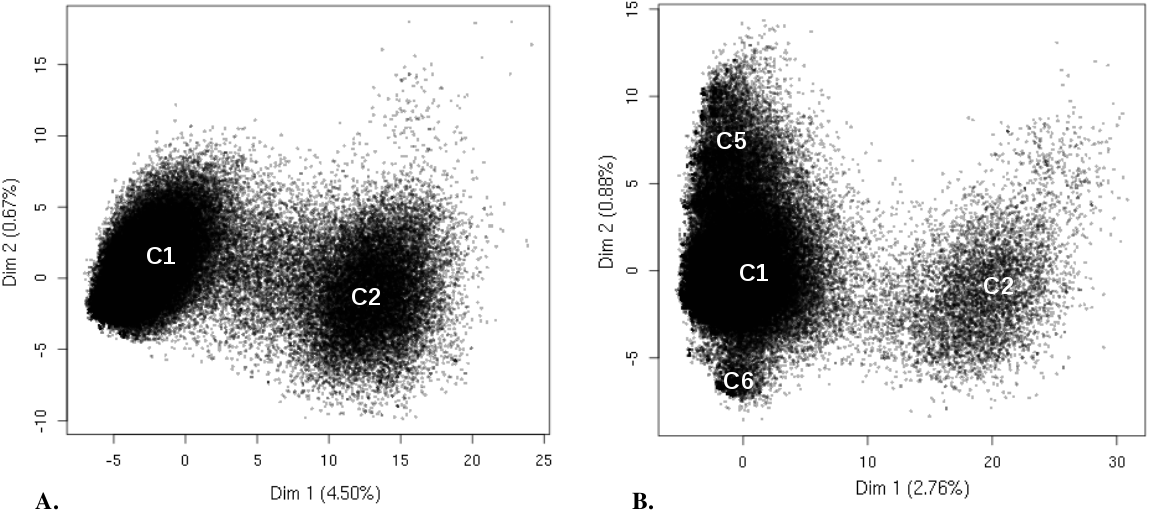
\includegraphics[scale=0.4]{img/ACP_experimental.png}  \\
		\caption{\textbf{Caractérisation visuelle des familles $\alpha$-satellite chez \textit{C. solatus} et \textit{C. pogonias}:}\label{fig:ACP_exp}
		Le nom des familles est indiqué sur les graphiques. Un point représente un monomère. \textbf{A.} Les familles présentes chez \textit{C. solatus}. \textbf{B.} Les familles présentes chez \textit{C. pogonias}.} 
	\end{figure}
	
			La classification automatisée donne des familles de taille variable allant de deux  à des dizaines de milliers de séquences. Seules les familles ayant plus de 100 séquences, appelées "grandes familles", sont conservées pour l'analyse des familles. Les "petites familles" sont prises en compte en terme de pourcentage de séquences qui ne figurent pas dans l'analyse. Les séquences $\alpha$-satellites chez \textit{solatus} sont réparties en 564 familles, dont 12 grandes familles. Les séquences qui ne sont pas retenues représentent 3,97\% du jeu de données. Chez pogonias, le nombre total de familles est de 132, avec 13 grandes familles et 1,29\% du jeu de données qui  ne figure pas dans les analyses.\\
			 Le nombre de grandes familles est relativement proche entre ces deux espèces, mais diffèrent significativement des résultats expérimentaux. Parmi ces dizaines de familles, chez \textit{C. solatus} 11 familles forment la famille C2, une familles forme la famille C1 et les familles C3 et C4 sont retrouvées dans des petites familles d'environ 80 séquences chacune. Toutes les familles sont retrouvées chez \textit{C. pogonias} sauf la famille C6. La famille C1 est composée de 10 familles, les familles C2, C3 et C5 sont composé d'une famille respectivement, et C4 correspond a une petite famille. Ces résultats contredisent les résultats expérimentaux. La famille C2 et censée être divisée en plusieurs groupes par ses séquences qui divergent plus que dans la famille 1.  
			 La classification expérimentale est une méthode visuelle basée sur l'ACP sur des 5-mers. Un point noir représente un monomère. Deux groupes distincts regroupent les familles C1 et C2 chez solatus et 4 groupes distincts sont retrouvés chez pogonias formant les familles C1, C2, C5 et C6. Sur cette représentation sont superposées les familles de la classification automatisée en couleur. \\
			 Le \textit{C. sabaeus} a 338 familles au total, dont 44 grandes familles, et 10,89\% du jeu de données qui n'est pas pris en compte. Le \textit{M. fascicularis} a respectivement 709 et 998 familles, dont 42 et 81 grandes familles, et 14,56\% et 5,05\% du jeu de données qui n'est pas pris en compte. Ces espèces ont beaucoup plus de grandes familles que les \textit{Cercopithèques}. 
			 
	\begin{figure}	
		\begin{tabular}{c} 
			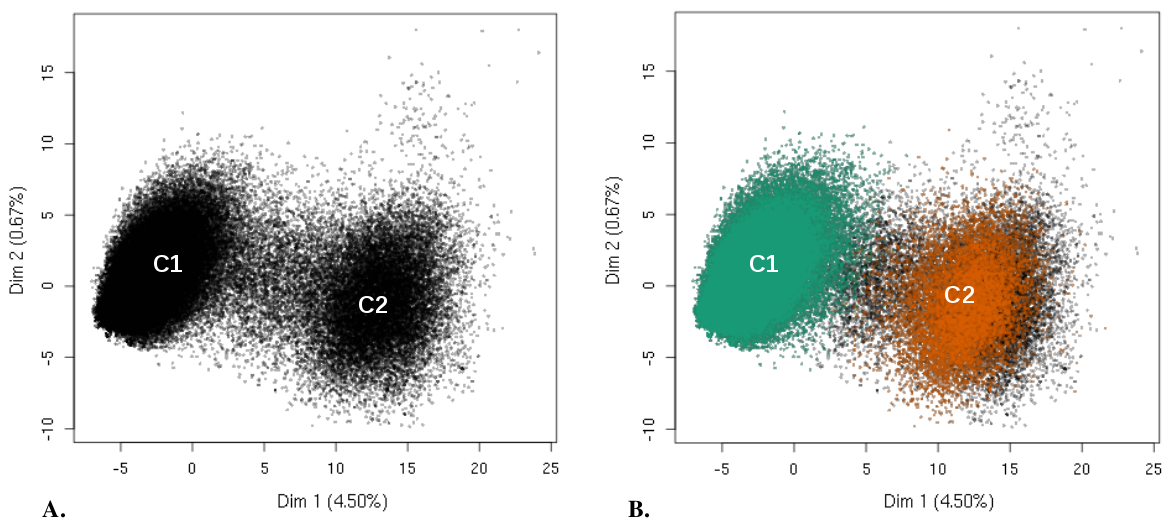
\includegraphics[scale=0.4]{img/ACP_solatus_1.png}  \\
			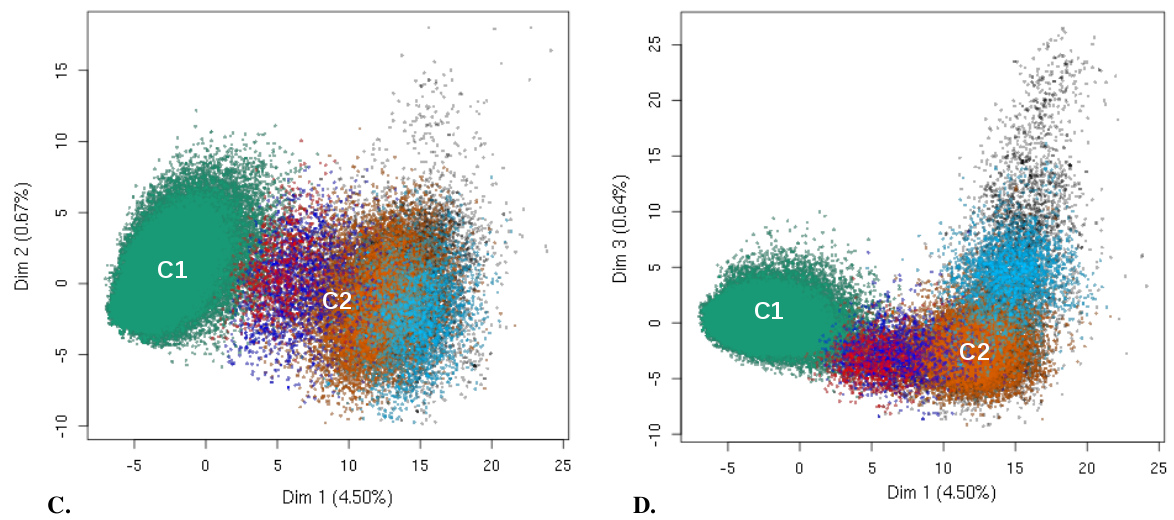
\includegraphics[scale=0.4]{img/ACP_solatus_2.png}  \\
		\end{tabular}
\caption{\textbf{Représentation de l'ACP des 5-mers chez \textit{C. solatus}:}
\label{fig:ACP_solatus}
Le nom des familles est indiqué sur les graphiques. Un point représente un monomère. \textbf{A.}Les familles expérimentales C1 et C2 sont en noir. Les résultats de la classification automatisée sont superposés en couleur aux résultats expérimentaux.\textbf{B.}Les familles C1 et C2 sont respectivement en vert et orange. \textbf{C.} Les familles C2 intermédiaires sont rajoutées au graphe. Les familles 2, 4 et 7 sont respectivement en  bleu, rouge et turquoise. \textbf{D.}} 
\end{figure}

		\begin{figure}	
		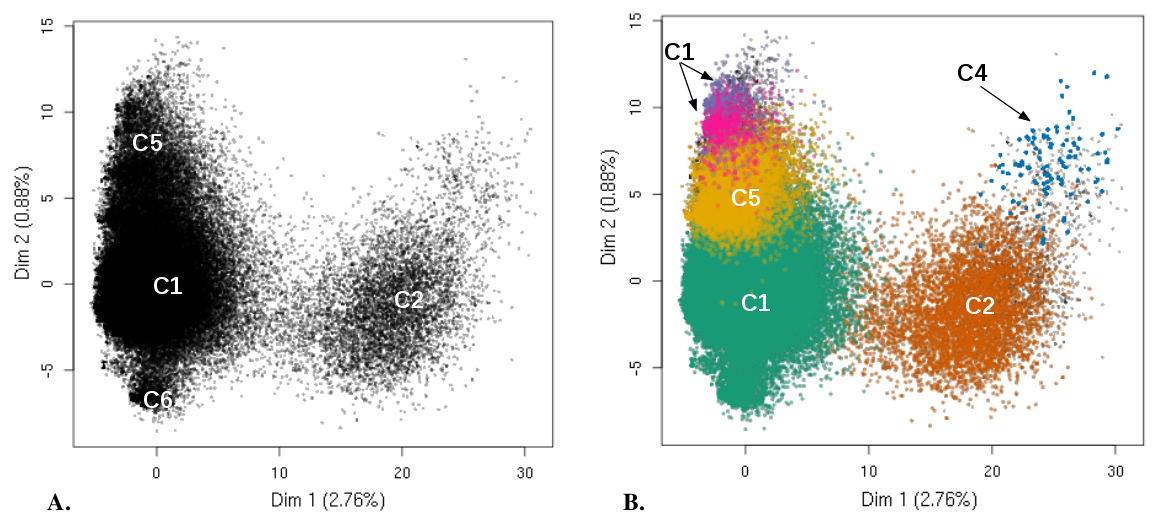
\includegraphics[scale=0.4]{img/ACP_pogonias_1.png}  \\
		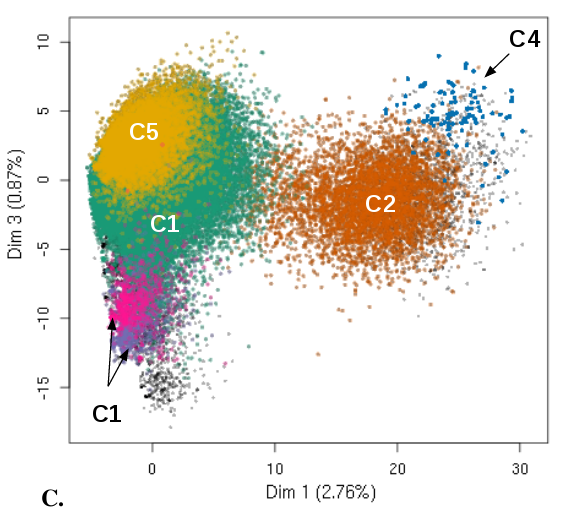
\includegraphics[scale=0.4]{img/ACP_pogonias_2.png}   \\
		\caption{\textbf{Représentation de l'ACP des 5-mers chez \textit{C. pogonias}:}
		\label{fig:ACP_pogonias}			
		Le nom des familles est indiqué sur les graphiques. Un point représente un monomère. \textbf{A.}Les familles expérimentales C1 et C2 sont en noir. Les résultats de la classification automatisée sont superposés en couleur aux résultats expérimentaux.\textbf{B.}Les familles C1 et C2 sont respectivement en vert et orange. \textbf{C.} Les familles C2 intermédiaires sont rajoutées au graphe. Les familles 2, 4 et 7 sont respectivement en  bleu, rouge et turquoise. \textbf{D.}} 
		\end{figure}
		
			\subsubsection{Motifs CENP-B, pJ$\alpha$ et pK$\beta$}
			\subsubsection{Similarité entre familles}
	
	\subsection{Comparaison inter-espèce et mécanismes d'évolution}


\section{Discussion}
\section{Conclusion}

\newpage
\strut  ~  \mbox{}  \null
\newpage

\bibliographystyle{plain} \bibliography{biblio} 

%
%	\makeindex % index général
%   \newindex{env}{enx}{end}{Environnements}
%   \newindex{ext}{exx}{exd}{Extensions}
%   \newindex{cmm}{cmx}{cmd}{Commandes}
%	\newcommand{\commande}[1]
%   {\texttt{\textbackslash #1}}
%	\newcommand{\indexcmm}[1]
%   {\index[cmm]{#1@\commande{#1}}} % index d'une commande
% 
%
%
%
%Une citation\index{citation} hors paragraphe
%se met dans un environnement
%\emph{quote}\index[env]{quote}
%ou \emph{quotation}\index[env]{quotation}
% 
%L'extension \emph{array}\index[ext]{array}
%fournit les commandes
%\commande{raggedleft}\indexcmm{raggedleft}
%et \commande{raggedright}\indexcmm{raggedright}.
% 
%\printindex % index général
%\printindex[env]
%\printindex[ext]
%\printindex[cmm]

%%%%%%%%%%%%%%%%%%%%%%%%%%%%%%%%%%%%%%%%%%%%%%%%%%%%%%%%%%%%%%%%%%
%%%%%%%%%%%%%%%%%%%%Résumé & Abstract%%%%%%%%%%%%%%%%%%%%%%%%%%%%%
%%%%%%%%%%%%%%%%%%%%%%%%%%%%%%%%%%%%%%%%%%%%%%%%%%%%%%%%%%%%%%%%%%
\newpage 
\thispagestyle{empty}
\section*{Résumé}~\\[0.2cm]
Votre résumé commence ici...
   ...
\section*{Abstract}~\\[0.2cm]
 Abstract begins here...
   ...
\end{document}
%
%%HELP: http://lataix-sebastien.developpez.com/tutoriels/latex/memoire-de-fin-d-etude/#LII-C